\RequirePackage{ifpdf}
\ifpdf\else\def\pgfsysdriver{pgfsys-dvisvgm.def}\fi
\documentclass[tikz,border=10pt]{standalone}
\usepackage[T1]{fontenc}
\usepackage{lmodern}
\usetikzlibrary{arrows.meta,backgrounds,calc}
\definecolor{blue}{HTML}{0072B2}
\definecolor{green}{HTML}{009E73}
\definecolor{orange}{HTML}{B44B00}
\definecolor{ink}{HTML}{243447}
\definecolor{gray}{HTML}{738294}
\tikzset{
 box/.style={draw=gray,rounded corners=3pt,text width=34mm,minimum height=14mm,align=center,text=ink,inner sep=5pt,font=\sffamily\small},
 actor/.style={box,text width=24mm,fill=white},
 component/.style={box,fill=blue!6},
 store/.style={box,fill=yellow!14},
 external/.style={box,fill=gray!7},
 panel/.style={fill=blue!2,draw=gray,rounded corners=5pt},
 flow/.style={-{Latex[length=2.5mm]},line width=1.25pt},
 run/.style={flow,draw=blue},
 again/.style={flow,draw=orange},
 grade/.style={flow,draw=green},
 relation/.style={draw=gray,dashed,line width=.85pt},
 label/.style={font=\sffamily\small,text=ink,align=center,fill=none,inner sep=2pt},
 heading/.style={font=\sffamily\bfseries,text=ink,anchor=west},
 title/.style={font=\sffamily\bfseries\Large,text=ink,anchor=west},
 note/.style={font=\sffamily\small,text=ink,anchor=west},
 every node/.append style={font=\sffamily}
}
\newcommand{\step}[2]{\tikz[baseline=(s.base)]\node[circle,fill=#1,text=white,inner sep=1.6pt,font=\sffamily\tiny\bfseries](s){#2};}

\begin{document}
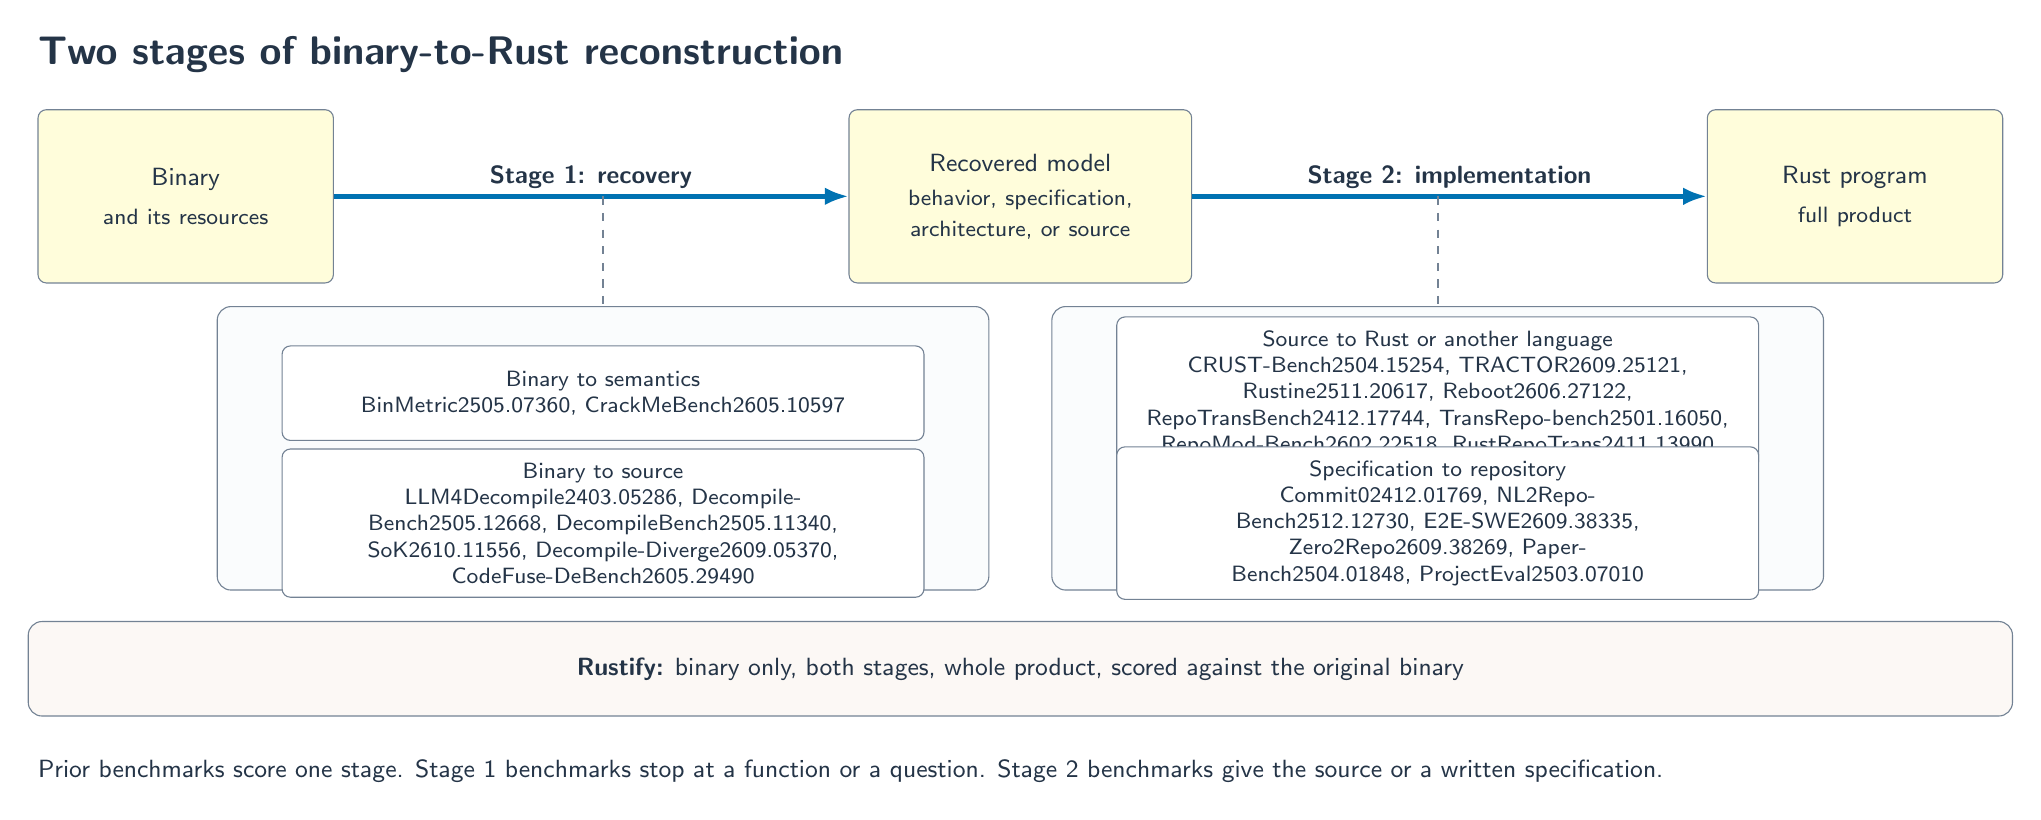
\begin{tikzpicture}[x=1cm,y=1cm]
 \tikzset{artifact/.style={box,fill=yellow!14,text width=34mm,minimum height=22mm},
  family/.style={box,fill=white,text width=78mm,minimum height=12mm,font=\sffamily\footnotesize},
  stage/.style={-{Latex[length=3mm]},line width=1.6pt,draw=blue}}
 \node[title] at (-0.6,7.8) {Two stages of binary-to-Rust reconstruction};
 \node[artifact] (binary) at (1.4,6.0) {Binary\\[3pt]\footnotesize and its resources};
 \node[artifact,text width=40mm] (model) at (12.0,6.0) {Recovered model\\[3pt]\footnotesize behavior, specification,\\\footnotesize architecture, or source};
 \node[artifact] (rust) at (22.6,6.0) {Rust program\\[3pt]\footnotesize full product};
 \draw[stage] (binary) -- node[label,above]{\textbf{Stage 1: recovery}} (model);
 \draw[stage] (model) -- node[label,above]{\textbf{Stage 2: implementation}} (rust);
 \draw[relation] (6.7,6.0) -- (6.7,4.6);
 \draw[relation] (17.3,6.0) -- (17.3,4.6);
 \node[family] (sem) at (6.7,3.5) {Binary to semantics\\\paper{BinMetric}{2505.07360}, \paper{CrackMeBench}{2605.10597}};
 \node[family] (dec) at (6.7,1.85) {Binary to source\\\paper{LLM4Decompile}{2403.05286}, \paper{Decompile-Bench}{2505.12668}, \paper{DecompileBench}{2505.11340},\\\paper{SoK}{2610.11556}, \paper{Decompile-Diverge}{2609.05370}, \paper{CodeFuse-DeBench}{2605.29490}};
 \node[family] (tra) at (17.3,3.5) {Source to Rust or another language\\\paper{CRUST-Bench}{2504.15254}, \paper{TRACTOR}{2609.25121}, \paper{Rustine}{2511.20617}, \paper{Reboot}{2606.27122},\\\paper{RepoTransBench}{2412.17744}, \paper{TransRepo-bench}{2501.16050},\\\paper{RepoMod-Bench}{2602.22518}, \paper{RustRepoTrans}{2411.13990}};
 \node[family] (gen) at (17.3,1.85) {Specification to repository\\\paper{Commit0}{2412.01769}, \paper{NL2Repo-Bench}{2512.12730}, \paper{E2E-SWE}{2609.38335},\\\paper{Zero2Repo}{2609.38269}, \paper{PaperBench}{2504.01848}, \paper{ProjectEval}{2503.07010}};
 \begin{scope}[on background layer]
  \filldraw[panel] (1.8,1.0) rectangle (11.6,4.6);
  \filldraw[panel] (12.4,1.0) rectangle (22.2,4.6);
  \filldraw[fill=orange!4,draw=gray,rounded corners=5pt] (-0.6,-0.6) rectangle (24.6,0.6);
 \end{scope}
 \node[font=\sffamily\small,text=ink] at (12.0,0.0) {\textbf{Rustify:} binary only, both stages, whole product, scored against the original binary};
 \node[note] at (-0.6,-1.3) {Prior benchmarks score one stage. Stage 1 benchmarks stop at a function or a question. Stage 2 benchmarks give the source or a written specification.};
\end{tikzpicture}
\end{document}
